\begin{figure}[H]
    \centering



\tikzset{every picture/.style={line width=0.75pt}} %set default line width to 0.75pt        

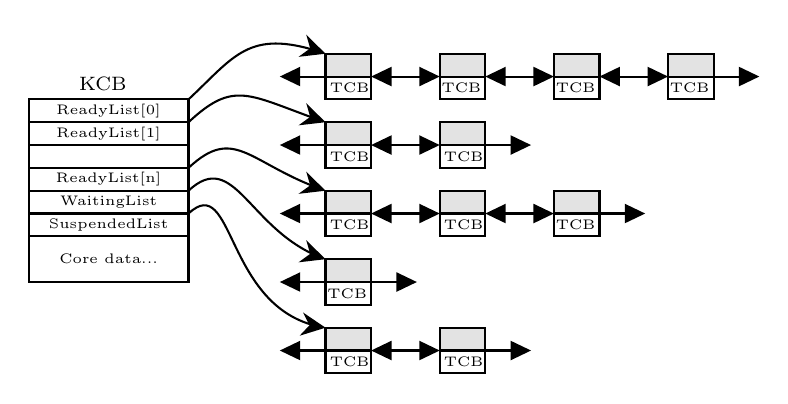
\begin{tikzpicture}[x=0.75pt,y=0.75pt,yscale=-1,xscale=1, scale=1.1]
%uncomment if require: \path (0,160.28571319580078); %set diagram left start at 0, and has height of 160.28571319580078

%Shape: Rectangle [id:dp15753116493869812] 
\draw   (70,30) -- (140,30) -- (140,40) -- (70,40) -- cycle ;
%Shape: Rectangle [id:dp4573538414066416] 
\draw   (70,70) -- (140,70) -- (140,80) -- (70,80) -- cycle ;
%Shape: Rectangle [id:dp19010756091304581] 
\draw   (70,80) -- (140,80) -- (140,90) -- (70,90) -- cycle ;
%Shape: Rectangle [id:dp5687118027525055] 
\draw   (70,40) -- (140,40) -- (140,50) -- (70,50) -- cycle ;
%Shape: Rectangle [id:dp3548324267311098] 
\draw   (70,60) -- (140,60) -- (140,70) -- (70,70) -- cycle ;
%Shape: Rectangle [id:dp38283546277399205] 
\draw   (70,50) -- (140,50) -- (140,60) -- (70,60) -- cycle ;
%Shape: Rectangle [id:dp8859203998363225] 
\draw   (70,90) -- (140,90) -- (140,110) -- (70,110) -- cycle ;
%Shape: Rectangle [id:dp8306955045955715] 
\draw   (200,10) -- (220,10) -- (220,30) -- (200,30) -- cycle ;
%Shape: Rectangle [id:dp43351283833138243] 
\draw   (250,10) -- (270,10) -- (270,30) -- (250,30) -- cycle ;
%Shape: Rectangle [id:dp040444176240501895] 
\draw  [fill={rgb, 255:red, 210; green, 210; blue, 210 }  ,fill opacity=0.62 ] (200,10) -- (220,10) -- (220,20) -- (200,20) -- cycle ;
%Shape: Rectangle [id:dp5261114839365322] 
\draw  [fill={rgb, 255:red, 210; green, 210; blue, 210 }  ,fill opacity=0.62 ] (250,10) -- (270,10) -- (270,20) -- (250,20) -- cycle ;
%Straight Lines [id:da7993610989249693] 
\draw    (223,20) -- (247,20) ;
\draw [shift={(250,20)}, rotate = 180] [fill={rgb, 255:red, 0; green, 0; blue, 0 }  ][line width=0.08]  [draw opacity=0] (8.93,-4.29) -- (0,0) -- (8.93,4.29) -- cycle    ;
\draw [shift={(220,20)}, rotate = 0] [fill={rgb, 255:red, 0; green, 0; blue, 0 }  ][line width=0.08]  [draw opacity=0] (8.93,-4.29) -- (0,0) -- (8.93,4.29) -- cycle    ;
%Shape: Rectangle [id:dp018852132251837128] 
\draw   (300,10) -- (320,10) -- (320,30) -- (300,30) -- cycle ;
%Shape: Rectangle [id:dp8577387789213544] 
\draw   (350,10) -- (370,10) -- (370,30) -- (350,30) -- cycle ;
%Shape: Rectangle [id:dp09544167255996117] 
\draw  [fill={rgb, 255:red, 210; green, 210; blue, 210 }  ,fill opacity=0.62 ] (300,10) -- (320,10) -- (320,20) -- (300,20) -- cycle ;
%Shape: Rectangle [id:dp4096099935237296] 
\draw  [fill={rgb, 255:red, 210; green, 210; blue, 210 }  ,fill opacity=0.62 ] (350,10) -- (370,10) -- (370,20) -- (350,20) -- cycle ;
%Straight Lines [id:da850104649119457] 
\draw    (323,20) -- (347,20) ;
\draw [shift={(350,20)}, rotate = 180] [fill={rgb, 255:red, 0; green, 0; blue, 0 }  ][line width=0.08]  [draw opacity=0] (8.93,-4.29) -- (0,0) -- (8.93,4.29) -- cycle    ;
\draw [shift={(320,20)}, rotate = 0] [fill={rgb, 255:red, 0; green, 0; blue, 0 }  ][line width=0.08]  [draw opacity=0] (8.93,-4.29) -- (0,0) -- (8.93,4.29) -- cycle    ;
%Straight Lines [id:da49162726200791584] 
\draw    (273,20) -- (297,20) ;
\draw [shift={(300,20)}, rotate = 180] [fill={rgb, 255:red, 0; green, 0; blue, 0 }  ][line width=0.08]  [draw opacity=0] (8.93,-4.29) -- (0,0) -- (8.93,4.29) -- cycle    ;
\draw [shift={(270,20)}, rotate = 0] [fill={rgb, 255:red, 0; green, 0; blue, 0 }  ][line width=0.08]  [draw opacity=0] (8.93,-4.29) -- (0,0) -- (8.93,4.29) -- cycle    ;
%Straight Lines [id:da5258969522636683] 
\draw    (370,20) -- (387,20) ;
\draw [shift={(390,20)}, rotate = 180] [fill={rgb, 255:red, 0; green, 0; blue, 0 }  ][line width=0.08]  [draw opacity=0] (8.93,-4.29) -- (0,0) -- (8.93,4.29) -- cycle    ;

%Straight Lines [id:da9297049530511214] 
\draw    (200,20) -- (183,20) ;
\draw [shift={(180,20)}, rotate = 360] [fill={rgb, 255:red, 0; green, 0; blue, 0 }  ][line width=0.08]  [draw opacity=0] (8.93,-4.29) -- (0,0) -- (8.93,4.29) -- cycle    ;

%Curve Lines [id:da41331111539282883] 
\draw    (140,30) .. controls (159.99,11.34) and (166.19,-0.95) .. (197.54,9.18) ;
\draw [shift={(200,10)}, rotate = 199.06] [fill={rgb, 255:red, 0; green, 0; blue, 0 }  ][line width=0.08]  [draw opacity=0] (10.72,-5.15) -- (0,0) -- (10.72,5.15) -- (7.12,0) -- cycle    ;

%Shape: Rectangle [id:dp42382431845225477] 
\draw   (200,40) -- (220,40) -- (220,60) -- (200,60) -- cycle ;
%Shape: Rectangle [id:dp4587195629312468] 
\draw   (250,40) -- (270,40) -- (270,60) -- (250,60) -- cycle ;
%Shape: Rectangle [id:dp044330486228031596] 
\draw  [fill={rgb, 255:red, 210; green, 210; blue, 210 }  ,fill opacity=0.62 ] (200,40) -- (220,40) -- (220,50) -- (200,50) -- cycle ;
%Shape: Rectangle [id:dp13520876908056811] 
\draw  [fill={rgb, 255:red, 210; green, 210; blue, 210 }  ,fill opacity=0.62 ] (250,40) -- (270,40) -- (270,50) -- (250,50) -- cycle ;
%Straight Lines [id:da18614605422872654] 
\draw    (223,50) -- (247,50) ;
\draw [shift={(250,50)}, rotate = 180] [fill={rgb, 255:red, 0; green, 0; blue, 0 }  ][line width=0.08]  [draw opacity=0] (8.93,-4.29) -- (0,0) -- (8.93,4.29) -- cycle    ;
\draw [shift={(220,50)}, rotate = 0] [fill={rgb, 255:red, 0; green, 0; blue, 0 }  ][line width=0.08]  [draw opacity=0] (8.93,-4.29) -- (0,0) -- (8.93,4.29) -- cycle    ;
%Straight Lines [id:da4753030984566553] 
\draw    (270,50) -- (287,50) ;
\draw [shift={(290,50)}, rotate = 180] [fill={rgb, 255:red, 0; green, 0; blue, 0 }  ][line width=0.08]  [draw opacity=0] (8.93,-4.29) -- (0,0) -- (8.93,4.29) -- cycle    ;

%Straight Lines [id:da7847403112637539] 
\draw    (200,50) -- (183,50) ;
\draw [shift={(180,50)}, rotate = 360] [fill={rgb, 255:red, 0; green, 0; blue, 0 }  ][line width=0.08]  [draw opacity=0] (8.93,-4.29) -- (0,0) -- (8.93,4.29) -- cycle    ;

%Curve Lines [id:da8961412082772617] 
\draw    (140,40) .. controls (159.99,21.34) and (166.19,28.07) .. (197.54,39.14) ;
\draw [shift={(200,40)}, rotate = 199.06] [fill={rgb, 255:red, 0; green, 0; blue, 0 }  ][line width=0.08]  [draw opacity=0] (10.72,-5.15) -- (0,0) -- (10.72,5.15) -- (7.12,0) -- cycle    ;

%Shape: Rectangle [id:dp3059275072741767] 
\draw   (200,70) -- (220,70) -- (220,90) -- (200,90) -- cycle ;
%Shape: Rectangle [id:dp0694969528251621] 
\draw   (250,70) -- (270,70) -- (270,90) -- (250,90) -- cycle ;
%Shape: Rectangle [id:dp3746672870799119] 
\draw  [fill={rgb, 255:red, 210; green, 210; blue, 210 }  ,fill opacity=0.62 ] (200,70) -- (220,70) -- (220,80) -- (200,80) -- cycle ;
%Shape: Rectangle [id:dp4758600257072063] 
\draw  [fill={rgb, 255:red, 210; green, 210; blue, 210 }  ,fill opacity=0.62 ] (250,70) -- (270,70) -- (270,80) -- (250,80) -- cycle ;
%Straight Lines [id:da855217932178395] 
\draw    (223,80) -- (247,80) ;
\draw [shift={(250,80)}, rotate = 180] [fill={rgb, 255:red, 0; green, 0; blue, 0 }  ][line width=0.08]  [draw opacity=0] (8.93,-4.29) -- (0,0) -- (8.93,4.29) -- cycle    ;
\draw [shift={(220,80)}, rotate = 0] [fill={rgb, 255:red, 0; green, 0; blue, 0 }  ][line width=0.08]  [draw opacity=0] (8.93,-4.29) -- (0,0) -- (8.93,4.29) -- cycle    ;
%Straight Lines [id:da5706715249029704] 
\draw    (200,80) -- (183,80) ;
\draw [shift={(180,80)}, rotate = 360] [fill={rgb, 255:red, 0; green, 0; blue, 0 }  ][line width=0.08]  [draw opacity=0] (8.93,-4.29) -- (0,0) -- (8.93,4.29) -- cycle    ;

%Curve Lines [id:da7148467106529148] 
\draw    (140,60) .. controls (159.99,41.34) and (166.19,57.57) .. (197.54,69.12) ;
\draw [shift={(200,70)}, rotate = 199.06] [fill={rgb, 255:red, 0; green, 0; blue, 0 }  ][line width=0.08]  [draw opacity=0] (10.72,-5.15) -- (0,0) -- (10.72,5.15) -- (7.12,0) -- cycle    ;

%Straight Lines [id:da3102328153591005] 
\draw    (273,80) -- (297,80) ;
\draw [shift={(300,80)}, rotate = 180] [fill={rgb, 255:red, 0; green, 0; blue, 0 }  ][line width=0.08]  [draw opacity=0] (8.93,-4.29) -- (0,0) -- (8.93,4.29) -- cycle    ;
\draw [shift={(270,80)}, rotate = 0] [fill={rgb, 255:red, 0; green, 0; blue, 0 }  ][line width=0.08]  [draw opacity=0] (8.93,-4.29) -- (0,0) -- (8.93,4.29) -- cycle    ;
%Shape: Rectangle [id:dp9418769513436311] 
\draw   (300,70) -- (320,70) -- (320,90) -- (300,90) -- cycle ;
%Shape: Rectangle [id:dp6080731585015813] 
\draw  [fill={rgb, 255:red, 210; green, 210; blue, 210 }  ,fill opacity=0.62 ] (300,70) -- (320,70) -- (320,80) -- (300,80) -- cycle ;
%Straight Lines [id:da4468666430650001] 
\draw    (320,80) -- (337,80) ;
\draw [shift={(340,80)}, rotate = 180] [fill={rgb, 255:red, 0; green, 0; blue, 0 }  ][line width=0.08]  [draw opacity=0] (8.93,-4.29) -- (0,0) -- (8.93,4.29) -- cycle    ;

%Shape: Rectangle [id:dp337686946882503] 
\draw   (200,100) -- (220,100) -- (220,120) -- (200,120) -- cycle ;
%Shape: Rectangle [id:dp7402813545483575] 
\draw  [fill={rgb, 255:red, 210; green, 210; blue, 210 }  ,fill opacity=0.62 ] (200,100) -- (220,100) -- (220,110) -- (200,110) -- cycle ;
%Straight Lines [id:da23056890627510018] 
\draw    (220,110) -- (237,110) ;
\draw [shift={(240,110)}, rotate = 180] [fill={rgb, 255:red, 0; green, 0; blue, 0 }  ][line width=0.08]  [draw opacity=0] (8.93,-4.29) -- (0,0) -- (8.93,4.29) -- cycle    ;

%Straight Lines [id:da8695559665648553] 
\draw    (200,110) -- (183,110) ;
\draw [shift={(180,110)}, rotate = 360] [fill={rgb, 255:red, 0; green, 0; blue, 0 }  ][line width=0.08]  [draw opacity=0] (8.93,-4.29) -- (0,0) -- (8.93,4.29) -- cycle    ;

%Curve Lines [id:da7092078875258845] 
\draw    (140,70) .. controls (159.99,51.34) and (166.19,86.59) .. (197.54,99.08) ;
\draw [shift={(200,100)}, rotate = 199.06] [fill={rgb, 255:red, 0; green, 0; blue, 0 }  ][line width=0.08]  [draw opacity=0] (10.72,-5.15) -- (0,0) -- (10.72,5.15) -- (7.12,0) -- cycle    ;

%Shape: Rectangle [id:dp6399207339428794] 
\draw   (200,130) -- (220,130) -- (220,150) -- (200,150) -- cycle ;
%Shape: Rectangle [id:dp37683132221131044] 
\draw   (250,130) -- (270,130) -- (270,150) -- (250,150) -- cycle ;
%Shape: Rectangle [id:dp6930255232212175] 
\draw  [fill={rgb, 255:red, 210; green, 210; blue, 210 }  ,fill opacity=0.62 ] (200,130) -- (220,130) -- (220,140) -- (200,140) -- cycle ;
%Shape: Rectangle [id:dp5692267719035351] 
\draw  [fill={rgb, 255:red, 210; green, 210; blue, 210 }  ,fill opacity=0.62 ] (250,130) -- (270,130) -- (270,140) -- (250,140) -- cycle ;
%Straight Lines [id:da2601556043579827] 
\draw    (223,140) -- (247,140) ;
\draw [shift={(250,140)}, rotate = 180] [fill={rgb, 255:red, 0; green, 0; blue, 0 }  ][line width=0.08]  [draw opacity=0] (8.93,-4.29) -- (0,0) -- (8.93,4.29) -- cycle    ;
\draw [shift={(220,140)}, rotate = 0] [fill={rgb, 255:red, 0; green, 0; blue, 0 }  ][line width=0.08]  [draw opacity=0] (8.93,-4.29) -- (0,0) -- (8.93,4.29) -- cycle    ;
%Straight Lines [id:da2895668265413387] 
\draw    (270,140) -- (287,140) ;
\draw [shift={(290,140)}, rotate = 180] [fill={rgb, 255:red, 0; green, 0; blue, 0 }  ][line width=0.08]  [draw opacity=0] (8.93,-4.29) -- (0,0) -- (8.93,4.29) -- cycle    ;

%Straight Lines [id:da004922990676545114] 
\draw    (200,140) -- (183,140) ;
\draw [shift={(180,140)}, rotate = 360] [fill={rgb, 255:red, 0; green, 0; blue, 0 }  ][line width=0.08]  [draw opacity=0] (8.93,-4.29) -- (0,0) -- (8.93,4.29) -- cycle    ;

%Curve Lines [id:da5018986217326571] 
\draw    (140,80) .. controls (160.09,61.24) and (155.69,120.96) .. (197.39,129.54) ;
\draw [shift={(200,130)}, rotate = 188.4] [fill={rgb, 255:red, 0; green, 0; blue, 0 }  ][line width=0.08]  [draw opacity=0] (10.72,-5.15) -- (0,0) -- (10.72,5.15) -- (7.12,0) -- cycle    ;


% Text Node
\draw (105,75) node  [font=\tiny] [align=left] {WaitingList};
% Text Node
\draw (105,85) node  [font=\tiny] [align=left] {SuspendedList};
% Text Node
\draw (105,35) node  [font=\tiny] [align=left] {ReadyList[0]};
% Text Node
\draw (105,45) node  [font=\tiny] [align=left] {ReadyList[1]};
% Text Node
\draw (105,65) node  [font=\tiny] [align=left] {ReadyList[n]};
% Text Node
\draw (105,100) node  [font=\tiny] [align=left] {Core data...};
% Text Node
\draw (102.5,23) node  [font=\scriptsize] [align=left] {KCB};
% Text Node
\draw (210.5,25) node  [font=\tiny] [align=left] {TCB};
% Text Node
\draw (259.5,25) node  [font=\tiny] [align=left] {TCB};
% Text Node
\draw (309.5,25) node  [font=\tiny] [align=left] {TCB};
% Text Node
\draw (359.5,25) node  [font=\tiny] [align=left] {TCB};
% Text Node
\draw (210.5,55) node  [font=\tiny] [align=left] {TCB};
% Text Node
\draw (260.5,55) node  [font=\tiny] [align=left] {TCB};
% Text Node
\draw (210.5,85) node  [font=\tiny] [align=left] {TCB};
% Text Node
\draw (260.5,85) node  [font=\tiny] [align=left] {TCB};
% Text Node
\draw (309.5,85) node  [font=\tiny] [align=left] {TCB};
% Text Node
\draw (209.5,115) node  [font=\tiny] [align=left] {TCB};
% Text Node
\draw (210.5,145) node  [font=\tiny] [align=left] {TCB};
% Text Node
\draw (260.5,145) node  [font=\tiny] [align=left] {TCB};


 \end{tikzpicture}

    \caption{OS lists}
    \label{fig:corelists}
\end{figure}